\documentclass[10pt,fleqn]{beamer}

\usepackage{multimedia}
\usepackage[normal,tabtopcap,figbotcap]{subfigure}
\usepackage{cite}
\usepackage{BeamerColor}


 \definecolor{seagreen}{rgb}{0.2,0.2,0.6}
 \definecolor{blue}{rgb}{0.2,0.2,0.6}
%%%%%%%%%%%%%%%%%%%%%%%%%%%%%%%%%%%%%%%%%%%%%%%%%%%%%%%%%%%%%%%%%%
%% Pr�ambel
%%%%%%%%%%%%%%%%%%%%%%%%%%%%%%%%%%%%%%%%%%%%%%%%%%%%%%%%%%%%%%%%%%

%% Folien-Template einstellen
\mode<presentation>
{
  \usepackage{beamerthemeEAD}
  \setbeamercovered{transparent}
}

%% set your language
\usepackage[english]{babel}
%\usepackage[ngerman]{babel}

%% encoding
\usepackage[latin1]{inputenc}
\usepackage[T1]{fontenc}

\usepackage{graphicx}
\setlength{\fboxsep}{0.0pt}
\setlength\fboxrule{0.5pt}
\usepackage{tikz}

% enth�lt die konfiguration f�r das listings package
\usepackage{listings}
\usepackage{xcolor}

\lstset{language=Java}
\definecolor{lst_light_grey}
{rgb}{0.95,0.95,0.95}

\definecolor{lst_dark_grey}
{rgb}{0.8,0.8,0.8}

\definecolor{lst_highlight}
{rgb}{0,0,0.6}

\definecolor{lstgreen}
{rgb}{0,0.6,0}

\definecolor{lstmauve}
{rgb}{0.58,0,0.82}

\lstset{ %
	basicstyle=\small\ttfamily, %
	backgroundcolor=\color{lst_light_grey}, %
	captionpos=b, %
	commentstyle=\color{lstgreen}, %
	frame=single, %
	tabsize=2, %
	%
	keywordstyle=\color{lst_highlight}, %
	%
	numbers=left, %
	%
	numberstyle=\scriptsize \color{lst_dark_grey}, %
	%
	rulecolor=\color{lst_dark_grey}, %
%	inputencoding=utf8
}

% additional highlighted keywords
\lstset { emph= {%
		var, function %
	}, emphstyle={\color{lst_highlight}}%
}
\lstset{literate=%
	{�}{{\"O}}1
	{�}{{\"A}}1
	{�}{{\"U}}1
	{�}{{\ss}}2
	{�}{{\"u}}1
	{�}{{\"a}}1
	{�}{{\"o}}1
	{�}{{\'a}}1
	{�}{{\~a}}1
	{�}{{\'e}}1 
}

\lstset{showstringspaces=false}


\setbeamercolor{blue}{fg=blue}
\setbeamercolor{red}{fg=red}
\setbeamercolor{green}{fg=green}

% Makro for extra page in front of each section
\AtBeginSection[]{
 \begin{frame}
  \begin{block}{}
   \begin{center}\vspace{0.5cm}
   \Large\textcolor{blue}{\insertsection}\vspace{0.5cm}
   \end{center}
  \end{block}
\end{frame}
}% AtBeginSection

%%%%%%%%%%%%%%%%%%%%%%%%%%%%%%%%%%%%%%%%%%%%%%%%%%%%%%%%%%%%%%%%%%
%% Set up basic informations about your presentation
%%%%%%%%%%%%%%%%%%%%%%%%%%%%%%%%%%%%%%%%%%%%%%%%%%%%%%%%%%%%%%%%%%

\title{Entwicklung eines Datenloggers f�r M-Bus und KNX auf der Basis des Rasberry Pi}
\subtitle{Verteidigung der Bachelorarbeit}
\author[Tom Schumann]{Tom Schumann}
\institute{University of Applied Sciences Zittau/G�rlitz}
\date[DD\,/\,MM\,/\,JJJJ]{25\textsuperscript{th}~09~2015}

\begin{document}
\maketitleframe

\setcounter{tocdepth}{1}
\section[Gliederung]{}
\begin{frame}
\frametitle{Gliederung}
  \begin{columns}
   \begin{column}{7.0cm}
    \renewcommand{\baselinestretch}{1.5}
    \normalsize
    \tableofcontents
    \renewcommand{\baselinestretch}{1.0}
    \normalsize
   \end{column}
   \hspace*{-1.3cm}
   \begin{column}{4.0cm}
%		\includegraphics[width=3.5cm]{images/Pi_2_Model_B.png}
   \end{column}
  \end{columns}
\end{frame}
% % % % % % % % % % % % % % % % % % % % % % % % % % % % % % % % % % % % % % % % % % % % % % % % % % % % % % % % % % % % % % % % % % % % % %
\section[Netztopologie]{Netztopologie}
\begin{frame}{Netztopologie}{Ein Perzeptron f�r ein Konzept}
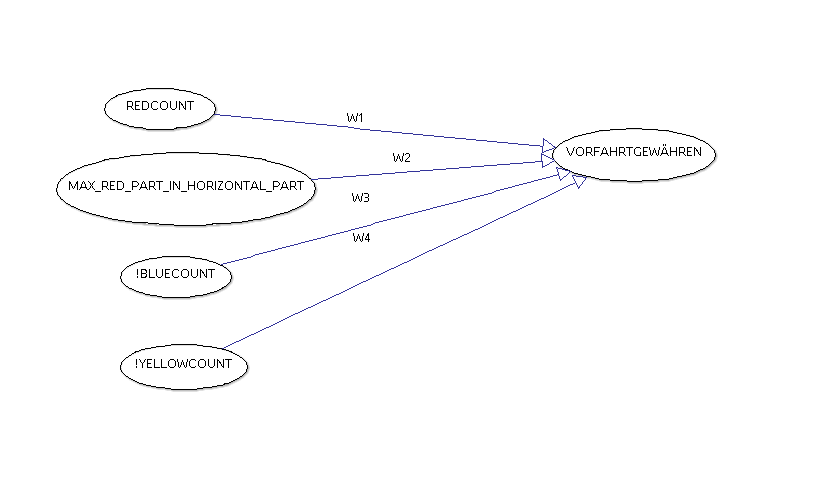
\includegraphics[scale=0.45]{images/vORFAHRTGEW.png}\\
\end{frame}

\begin{frame}{Netztopologie}{Bin�rcodierung der Konzept}
	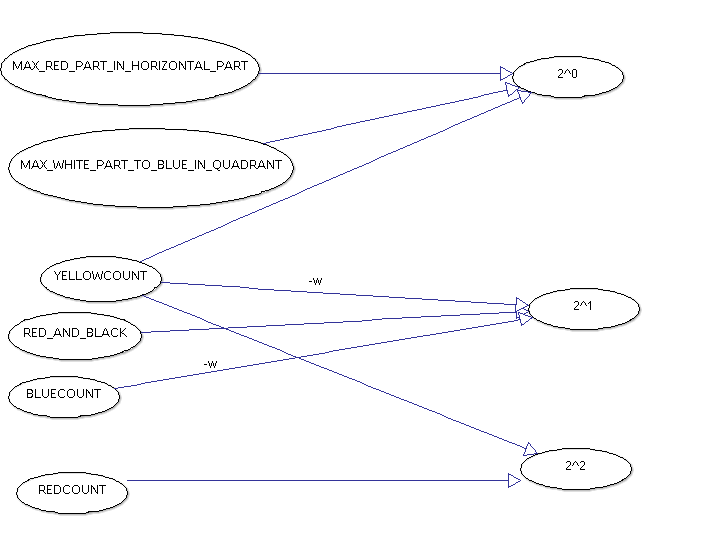
\includegraphics[scale=0.40]{images/bin.png}\\
\end{frame}


\section{Questions?}
\frame
{
\begin{center}
\frametitle{Fragen und Diskusion}
Vielen Dank f�r die Aufmerksamkeit.\\
\vspace*{0.4cm}
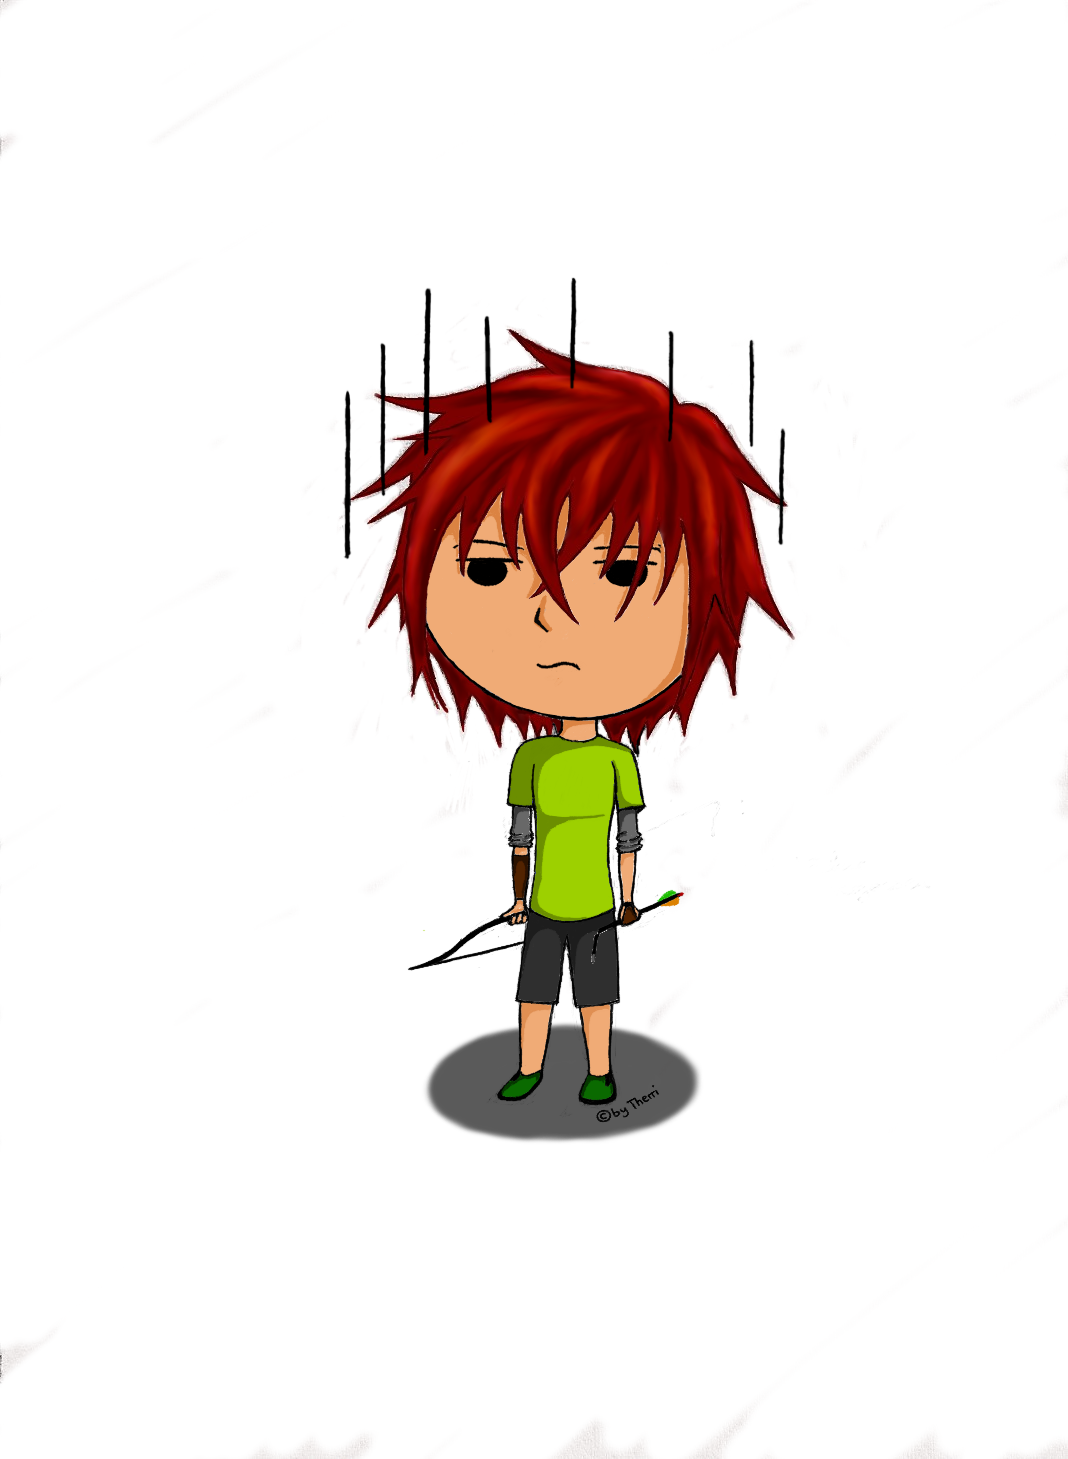
\includegraphics[scale=0.15]{images/fragen.png}\\
\vspace*{0.2cm}
Any questions?\\
\end{center}
}
\end{document}


